
\documentclass[border=6pt]{standalone}
\usepackage{pgfplots}
\pgfplotsset{compat=1.18}
\definecolor{adamw}{HTML}{0072B2}
\definecolor{muon}{HTML}{D55E00}
\begin{document}
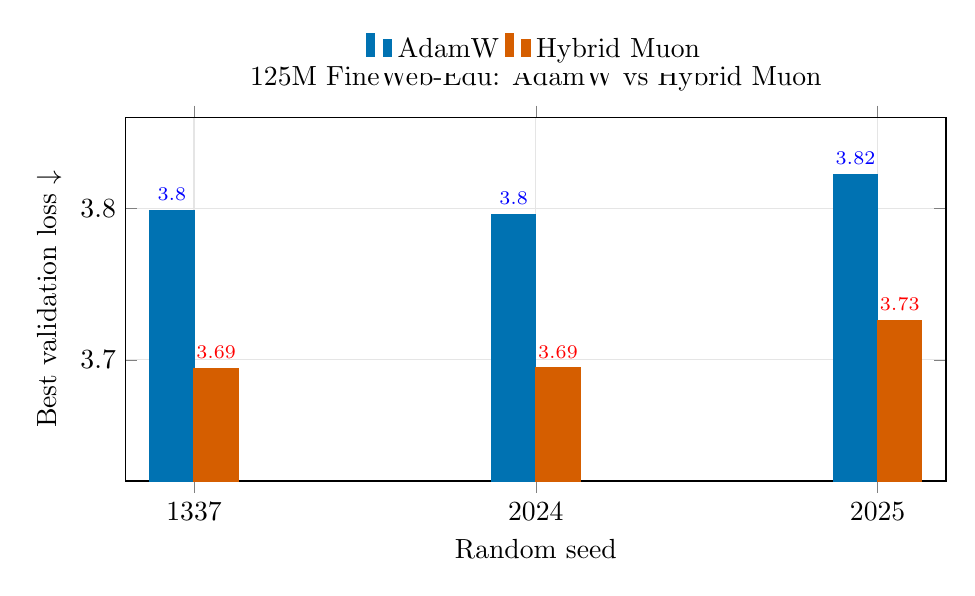
\begin{tikzpicture}
\begin{axis}[
    width=12cm,height=6.2cm,
    ybar=0pt,
    bar width=16pt,
    ymin=3.62,ymax=3.86,
    ylabel={Best validation loss $\downarrow$},
    xlabel={Random seed},
    title={125M FineWeb-Edu: AdamW vs Hybrid Muon},
    symbolic x coords={1337,2024,2025},
    xtick=data,
    xticklabels={1337,2024,2025},
    grid=major,
    grid style={black!10},
    legend style={draw=none, at={(0.5,1.12)}, anchor=south, legend columns=2},
    nodes near coords,
    every node near coord/.append style={font=\scriptsize, rotate=0, anchor=south},
]
\addplot+[fill=adamw, draw=adamw] coordinates {(1337,3.798632) (2024,3.795776) (2025,3.822396)};
\addlegendentry{AdamW}
\addplot+[fill=muon, draw=muon] coordinates {(1337,3.694427) (2024,3.694577) (2025,3.725771)};
\addlegendentry{Hybrid Muon}
\end{axis}
\end{tikzpicture}
\end{document}
